% =======================================================================
% Perpetual vs Spot: Is BTC Perpetual Funding a Harvestable Carry?
% Author: Dan Allouche
% =======================================================================
% All numeric values are loaded from numbers.tex, produced by
% scripts/report_numbers.py running the same pipeline as the notebooks.
% Build:  pdflatex report.tex && pdflatex report.tex
% =======================================================================

\documentclass[11pt]{article}

\usepackage[a4paper,margin=2.4cm]{geometry}
\usepackage[T1]{fontenc}
\usepackage{lmodern}
\usepackage[utf8]{inputenc}
\usepackage{amsmath, amssymb}
\usepackage{booktabs}
\usepackage{graphicx}
\usepackage{caption}
\usepackage{xcolor}
\usepackage{hyperref}
\usepackage{enumitem}
\usepackage{float}

\hypersetup{colorlinks=true, linkcolor=blue!50!black, citecolor=blue!50!black, urlcolor=blue!60!black}
\setlist[itemize]{leftmargin=*, itemsep=2pt, topsep=2pt}
\graphicspath{{../docs/figures/}}
\captionsetup{font=small, labelfont=bf}
% Auto-generated by scripts/report_numbers.py — do not edit by hand.
\newcommand{\dataStart}{2021-01-01}
\newcommand{\dataEnd}{2024-12-31}
\newcommand{\nBars}{1,461}
\newcommand{\nSymbols}{3}
\newcommand{\caseStart}{2024-01-01}
\newcommand{\caseEnd}{2024-03-20}
\newcommand{\spotRet}{+60.2\%}
\newcommand{\spotSharpe}{3.78}
\newcommand{\spotSortino}{4.04}
\newcommand{\spotMdd}{-15.8\%}
\newcommand{\spotFund}{\$0}
\newcommand{\perpRet}{+215.2\%}
\newcommand{\perpSharpe}{3.85}
\newcommand{\perpSortino}{4.11}
\newcommand{\perpMdd}{-50.5\%}
\newcommand{\perpFund}{\$261}
\newcommand{\carryRet}{+6.2\%}
\newcommand{\carrySharpe}{15.15}
\newcommand{\carrySortino}{10.96}
\newcommand{\carryMdd}{-0.3\%}
\newcommand{\carryFund}{\$65}
\newcommand{\breakeven}{169.5\%}
\newcommand{\nQuarters}{16}
\newcommand{\wfCarryMed}{+2.2\%}
\newcommand{\wfCarryWorst}{+0.4\%}
\newcommand{\wfCarrySharpe}{9.09}
\newcommand{\wfCarryMdd}{-0.5\%}
\newcommand{\wfCarryLiq}{0}
\newcommand{\wfPerpMed}{-3.1\%}
\newcommand{\wfPerpWorst}{-100.0\%}
\newcommand{\wfPerpSharpe}{1.08}
\newcommand{\wfPerpMdd}{-100.0\%}
\newcommand{\wfPerpLiq}{3}
\newcommand{\wfSpotMed}{+3.0\%}
\newcommand{\wfSpotWorst}{-56.4\%}
\newcommand{\wfSpotSharpe}{0.48}
\newcommand{\wfSpotMdd}{-59.4\%}
\newcommand{\wfSpotLiq}{0}
\newcommand{\carryFullRet}{+94.2\%}
\newcommand{\carryFullSharpe}{8.84}
\newcommand{\carryFullMdd}{-0.3\%}
\newcommand{\carryFullFund}{\$943}
\newcommand{\fundingAPR}{13.6\%}
\newcommand{\levelCorr}{0.999999}
\newcommand{\returnCorr}{0.999964}
\newcommand{\basisMean}{-1.03}
\newcommand{\basisStd}{5.41}
\newcommand{\basisHL}{4.8}
\newcommand{\adfP}{\ensuremath{3.2\times10^{-5}}}
\newcommand{\cointP}{0.013}
\newcommand{\kurtosis}{3.41}
\newcommand{\jbP}{\ensuremath{1.8\times10^{-155}}}
\newcommand{\annVol}{62.1\%}
\newcommand{\multiAssetBody}{BTC & +3.0\% & -3.1\% & +2.2\% & 3 \\
ETH & +20.3\% & +46.5\% & +2.5\% & 3 \\
SOL & +16.6\% & +31.2\% & +1.4\% & 6 \\}


\title{\textbf{Perpetual vs Spot: Is Bitcoin Perpetual Funding a Harvestable Carry?}}
\author{Dan Allouche}
\date{\today}

\begin{document}
\maketitle

\begin{abstract}
\noindent A long position on a perpetual futures contract continuously pays (or
receives) \emph{funding}. Viewed as a cost on a leveraged directional bet, funding
merely erodes returns; viewed as a cash flow on a market-neutral book, it is a
carry. Using daily Binance data for BTC, ETH and SOL over \dataStart{} to
\dataEnd{}, this study compares three books --- a spot long, a $4\times$ leveraged
perpetual long, and a delta-neutral cash-and-carry (long spot, short perpetual) ---
on a daily mark-to-market basis with a maintenance-margin liquidation guard. Over a
walk-forward across \nQuarters{} non-overlapping quarters, the $4\times$ perpetual
long has a \emph{negative} median quarterly return (\wfPerpMed{}) and is liquidated
in \wfPerpLiq{} quarters, whereas the delta-neutral carry is profitable in every
quarter (median \wfCarryMed{}, median Sharpe \wfCarrySharpe{}, worst drawdown
\wfCarryMdd{}) by harvesting a funding rate that averages \fundingAPR{} annualized.
The central finding is that, on a risk-adjusted and out-of-sample basis, the edge
is the funding carry, not the leverage.
\end{abstract}

\section{Introduction}
Perpetual futures (``perps'') are the dominant instrument in crypto derivatives.
Unlike dated futures they never expire; instead, a periodic \emph{funding} payment
exchanged between longs and shorts tethers the perpetual price to spot. When the
perp trades at a premium, longs pay shorts, and vice versa. A natural question for
a directional trader is how much this funding erodes a leveraged long. A more
interesting question for a systematic desk is whether the funding stream is itself
a tradable source of return.

This report answers both. We frame three books and evaluate them not on a single
hand-picked window but across multiple market regimes, with risk-adjusted metrics
and an explicit liquidation model. We deliberately avoid two common pitfalls: (i)
arguing ``market integration'' from the correlation of price \emph{levels}, which
is spurious for trending series \cite{yule1926,grangernewbold1974}; and (ii)
comparing raw returns across strategies that run at different leverage.

\section{Data}
All series are daily and sourced from Binance's public, geo-neutral historical
archive (\href{https://data.binance.vision}{data.binance.vision}): spot and
USDT-margined perpetual klines, and the 8-hour funding rate joined to the mark
price at each settlement. The snapshot covers \nSymbols{} symbols (BTC, ETH, SOL)
over \dataStart{}--\dataEnd{} (\nBars{} daily bars per symbol, three funding
settlements per day), and is committed to the repository so every result
reproduces offline. BTC is the primary symbol; ETH and SOL are used to test
generalization.

\section{Methodology}

\paragraph{Market integration.} Let $b_t = P^{\text{perp}}_t - P^{\text{spot}}_t$
be the basis. Integration is assessed by (i) the correlation of daily
\emph{returns}; (ii) the basis in basis points, its mean-reversion half-life from
an AR(1) fit, and an Augmented Dickey--Fuller (ADF) stationarity test; and (iii) an
Engle--Granger cointegration test on the two price levels \cite{englegranger1987}.

\paragraph{Books.} With investment (margin) $M$ and leverage $L$, the perpetual
position size is $q = M L / P^{\text{perp}}_0$ asset units. Each book is marked to
market daily:
\begin{itemize}
  \item \textbf{Spot $1\times$:} buy $M / P^{\text{spot}}_0$ units, hold.
  \item \textbf{Perp $L\times$:} equity $= M + q\,(P^{\text{perp}}_t - P^{\text{perp}}_0)
        - \text{funding}_t - \text{fees}$, with $L = 4$.
  \item \textbf{Carry ($\Delta$-neutral):} long $M/P^{\text{spot}}_0$ units of spot,
        short the same notional of perp. Net price exposure is the basis only; the
        short perp leg \emph{receives} funding.
\end{itemize}

\paragraph{Funding accrual.} Funding is summed strictly inside the holding window
$(t_{\text{open}}, t_{\text{close}}]$, charged on the live notional:
\[
\text{funding} = \sum_i r_i \cdot P^{\text{mark}}_i \cdot q,
\]
where $r_i$ is the 8-hour rate. A positive rate is a cost for a long and income for
the short carry leg; the sign is handled by arithmetic, so no regime needs special
casing. Reported as an annualized rate, funding is quoted on \emph{notional}, not
on the posted margin.

\paragraph{Risk and liquidation.} Metrics are computed on the daily equity path:
annualized Sharpe and Sortino, maximum drawdown, Calmar, historical VaR/CVaR and
hit rate. A maintenance-margin guard liquidates the leveraged book (capping its
loss at the margin) whenever equity falls below $m \cdot$ notional, so the path
risk that endpoint-only P\&L hides becomes visible.

\paragraph{Out-of-sample.} Books are run over \nQuarters{} non-overlapping
calendar quarters spanning bull, bear and sideways regimes; results are reported
as distributions, with a stationary block bootstrap for confidence intervals.

\section{Market structure}
Correlating the two price \emph{levels} gives \levelCorr{}, but this is mechanical:
both series share a trend, so the number is near one regardless of how tightly the
markets are linked. The economically meaningful quantity, the correlation of daily
\emph{returns}, is \returnCorr{}. Integration is better shown by the basis itself:
it averages \basisMean{}~bp (s.d.\ \basisStd{}~bp) with a mean-reversion half-life
of \basisHL{}~days, ADF rejects a unit root ($p = \adfP$), and the price levels are
cointegrated ($p = \cointP$). Daily returns are emphatically \emph{not} Gaussian:
excess kurtosis is \kurtosis{} and Jarque--Bera gives $p = \jbP$ --- fat tails that
make naive volatility and VaR understate downside, and that justify the liquidation
model for leverage. Annualized volatility is \annVol{}.

\begin{figure}[H]
\centering
\begin{minipage}{0.49\textwidth}\centering
  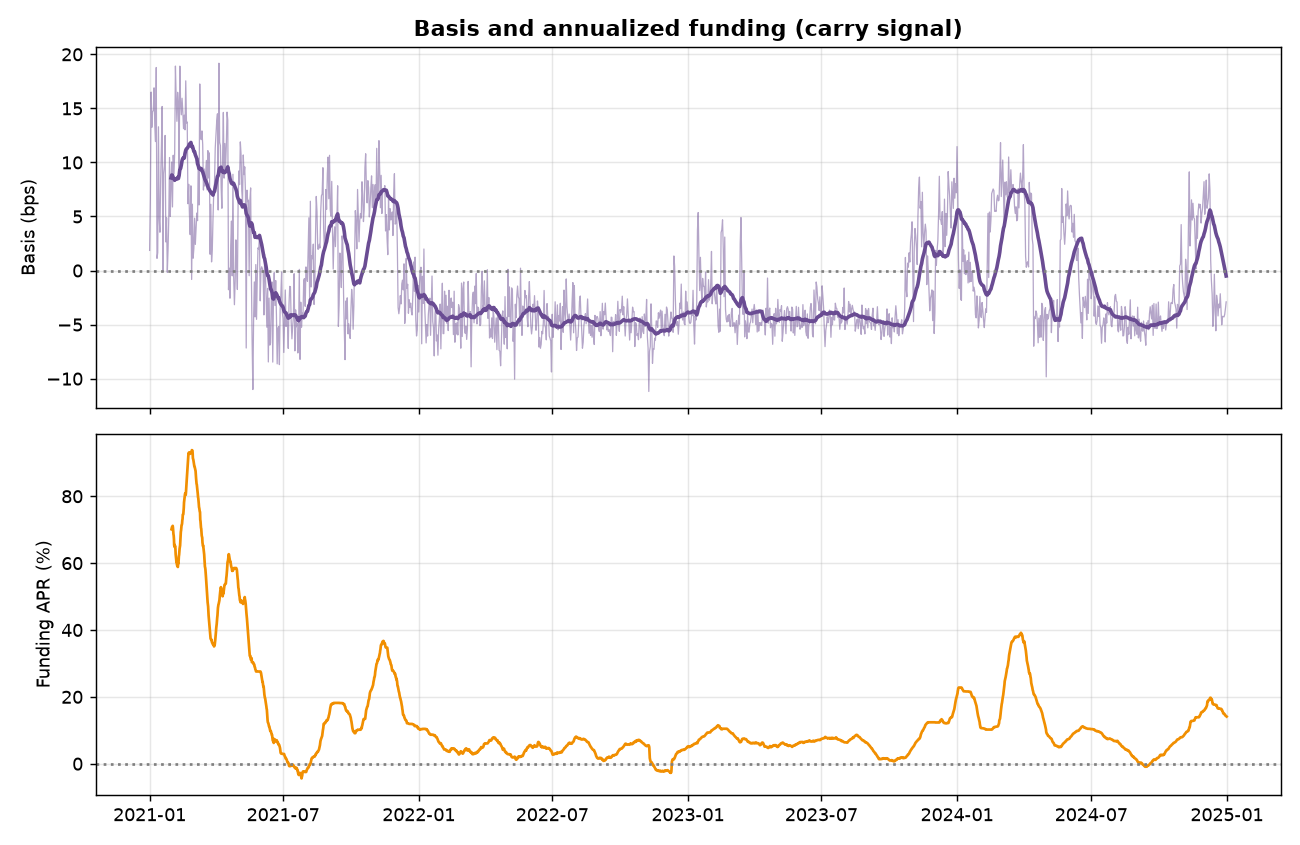
\includegraphics[width=\linewidth]{basis_funding.png}
\end{minipage}\hfill
\begin{minipage}{0.49\textwidth}\centering
  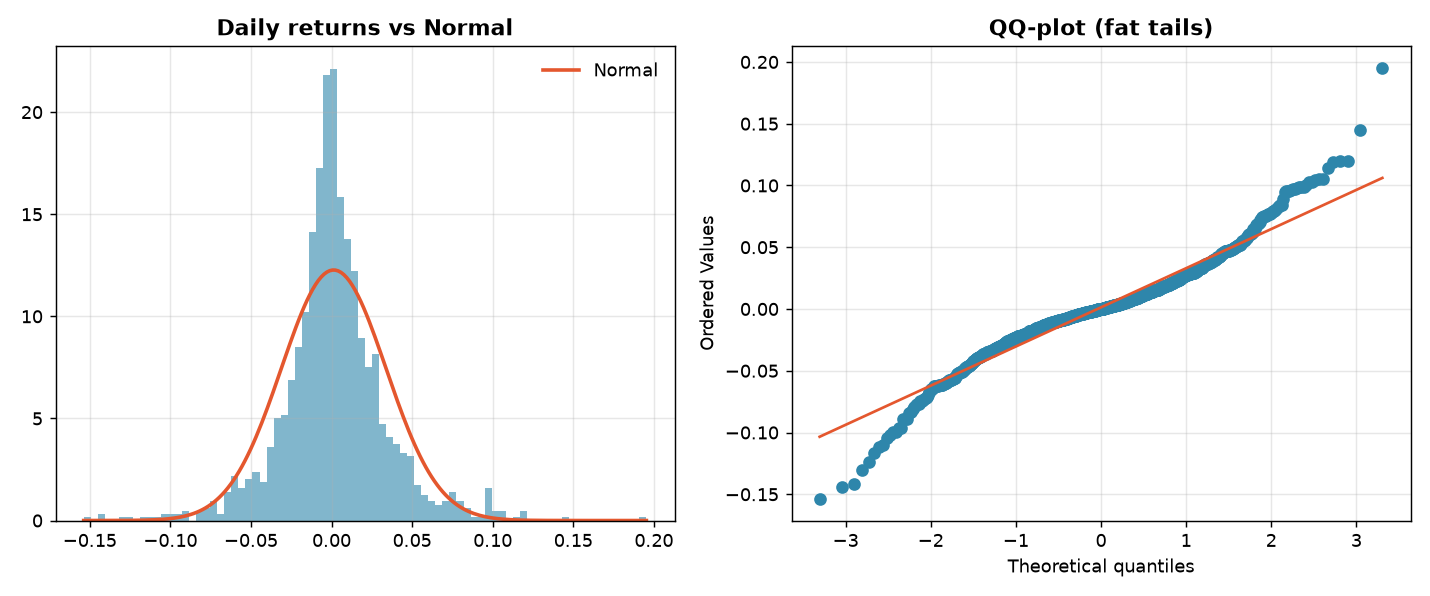
\includegraphics[width=\linewidth]{return_distribution.png}
\end{minipage}
\caption{Left: the perp--spot basis (top) and rolling annualized funding (bottom),
a positioning/carry signal. Right: the daily-return distribution and QQ-plot,
showing heavy tails relative to the normal.}
\end{figure}

\section{Strategy results}

\subsection{A single-window case study}
Over the 2024-Q1 window (\caseStart{} to \caseEnd{}, $M = \$1{,}000$, $L = 4$):

\begin{table}[H]\centering
\begin{tabular}{lrrrr}
\toprule
Strategy & Return & Sharpe & Max DD & Funding \\
\midrule
Spot $1\times$ & \spotRet & \spotSharpe & \spotMdd & \spotFund \\
Perp $4\times$ & \perpRet & \perpSharpe & \perpMdd & \perpFund \\
Carry ($\Delta$-neutral) & \carryRet & \carrySharpe & \carryMdd & \carryFund \\
\bottomrule
\end{tabular}
\caption{Case-study window. Leverage scales return and volatility together, so the
$4\times$ Sharpe ($\approx$ spot) buys no risk-adjusted edge while drawdown scales
$\sim$3$\times$. Funding would need to reach \breakeven{} APR to erase the leverage
edge in this window --- yet out of sample (below) leverage still loses.}
\end{table}

\subsection{The carry across the full history}
Held continuously over \dataStart{}--\dataEnd{}, the delta-neutral carry returns
\carryFullRet{} (Sharpe \carryFullSharpe{}, max drawdown \carryFullMdd{}),
accumulating \carryFullFund{} of funding income on \$1{,}000 of capital with
near-zero price exposure.

\subsection{Out-of-sample, across regimes}
Across all \nQuarters{} non-overlapping quarters:

\begin{table}[H]\centering
\begin{tabular}{lrrrrr}
\toprule
Strategy & Median & Worst & Med. Sharpe & Worst DD & Liquidations \\
\midrule
Carry ($\Delta$-neutral) & \wfCarryMed & \wfCarryWorst & \wfCarrySharpe & \wfCarryMdd & \wfCarryLiq{} / \nQuarters \\
Perp $4\times$ & \wfPerpMed & \wfPerpWorst & \wfPerpSharpe & \wfPerpMdd & \wfPerpLiq{} / \nQuarters \\
Spot $1\times$ & \wfSpotMed & \wfSpotWorst & \wfSpotSharpe & \wfSpotMdd & \wfSpotLiq{} / \nQuarters \\
\bottomrule
\end{tabular}
\caption{Walk-forward distribution of quarterly outcomes. The $4\times$ perp has a
negative median and is liquidated in \wfPerpLiq{} of \nQuarters{} quarters; the
carry is tight, positive and never liquidated.}
\end{table}

\begin{figure}[H]
\centering
\begin{minipage}{0.52\textwidth}\centering
  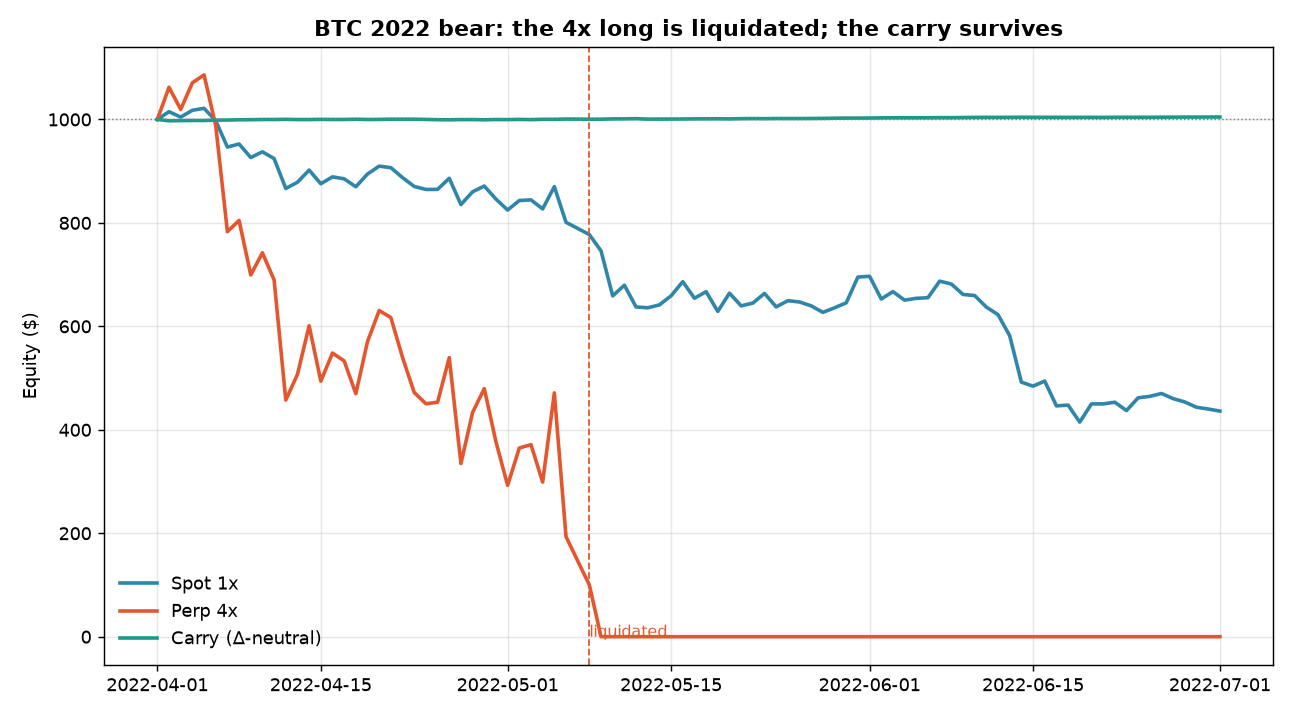
\includegraphics[width=\linewidth]{equity_bear.png}
\end{minipage}\hfill
\begin{minipage}{0.46\textwidth}\centering
  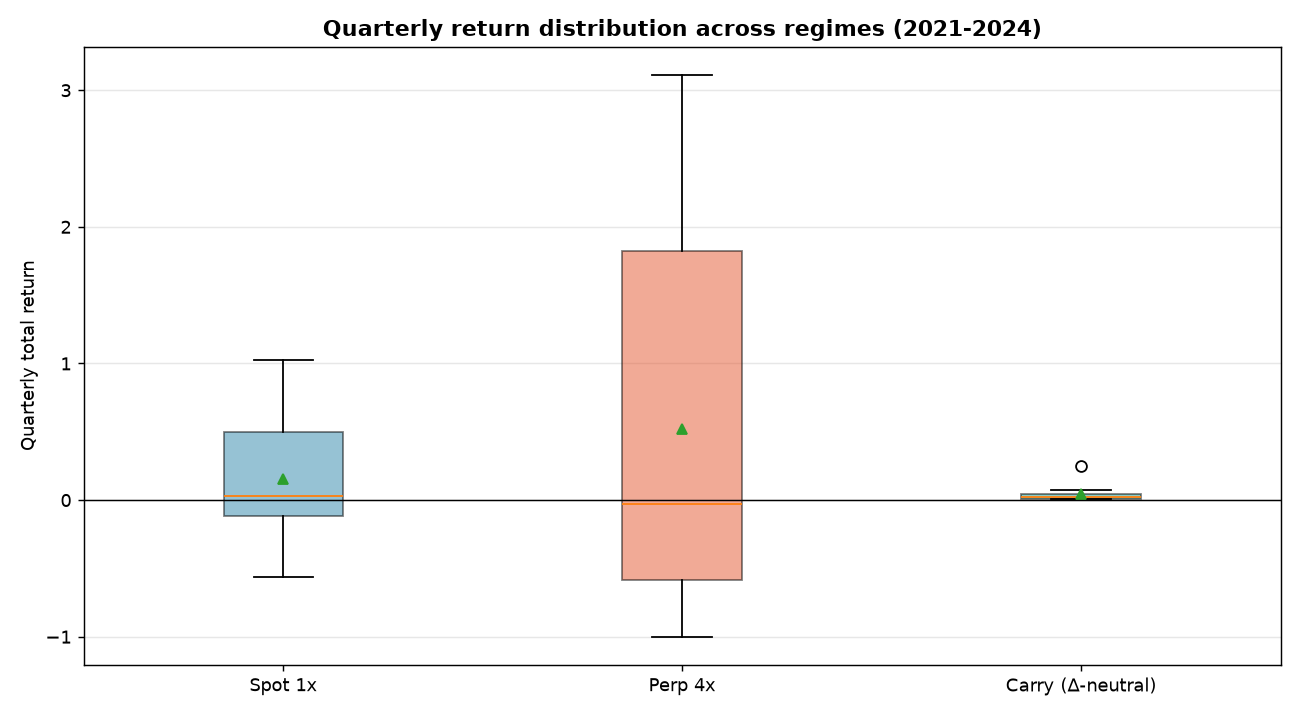
\includegraphics[width=\linewidth]{walkforward.png}
\end{minipage}
\caption{Left: the 2022 bear quarter --- the $4\times$ long is liquidated while the
carry is unscathed. Right: the distribution of quarterly returns by strategy; the
carry's box is a tight sliver above zero.}
\end{figure}

\subsection{Generalization to ETH and SOL}
The pattern is not BTC-specific. Median quarterly returns and $4\times$ liquidation
counts by symbol:

\begin{table}[H]\centering
\begin{tabular}{lrrrr}
\toprule
Symbol & Spot $1\times$ & Perp $4\times$ & Carry & Perp liq.\\
\midrule
\multiAssetBody
\bottomrule
\end{tabular}
\caption{For high-momentum alts the leveraged long can have a positive median, but
it is still liquidated several times; the carry stays positive and is never
liquidated.}
\end{table}

\section{Discussion}
Three points follow. First, ``leverage beats spot'' is true by construction in an
up-window --- a $4\times$ long's gross return is mechanically four times the spot
return --- and reverses in any down-window, so it is not a finding. Second, on a
risk-adjusted basis leverage is roughly Sharpe-neutral (it scales numerator and
denominator together) while it multiplies drawdown and adds liquidation risk;
unconditionally, the $4\times$ book is a coin flip that blows up about one quarter
in five. Third, the funding stream the directional trader pays is, for a
market-neutral book, a double-digit-APR carry harvested at a fraction of the
directional drawdown and with near-zero beta. The positive, persistent funding is
itself a signal: it reflects crowded longs paying to be long.

\section{Limitations}
Funding APR figures assume the 8-hour schedule (exact for BTC; some ETH/SOL periods
used a 4-hour schedule and are approximate). The liquidation guard is a simplified
flat maintenance-margin check, not a tick-level engine. Round-trip taker fees are
charged on notional, but slippage, partial fills, borrow constraints on the spot
leg, and the funding impact of the position itself are not modelled; the carry
assumes the short-perp leg is always fundable. Results are historical and
regime-dependent --- funding compresses, and can invert, in bear markets.

\section{Conclusion}
Comparing a spot long, a leveraged perpetual long and a delta-neutral funding carry
across multiple regimes and three assets, with daily mark-to-market and an explicit
liquidation model, the leveraged long offers no risk-adjusted edge and is
periodically wiped out, while the delta-neutral carry turns the same funding stream
into a stable, double-digit-APR return. The edge is the carry, not the leverage.

\begin{thebibliography}{9}
\small
\bibitem{yule1926} G.~U. Yule (1926). Why do we sometimes get nonsense-correlations
between time-series? \emph{J. Royal Statistical Society}, 89(1), 1--63.
\bibitem{grangernewbold1974} C.~W.~J. Granger and P. Newbold (1974). Spurious
regressions in econometrics. \emph{Journal of Econometrics}, 2(2), 111--120.
\bibitem{englegranger1987} R.~F. Engle and C.~W.~J. Granger (1987). Co-integration
and error correction. \emph{Econometrica}, 55(2), 251--276.
\bibitem{sharpe1994} W.~F. Sharpe (1994). The Sharpe ratio. \emph{Journal of
Portfolio Management}, 21(1), 49--58.
\end{thebibliography}

\end{document}
